% Authoritative, self-contained source. Compile with pdfLaTeX twice,
% or: latexmk -pdf consequences-of-binary-necklaces.tex
% All figures and references are embedded; no external assets are required.
\documentclass[11pt]{article}
\usepackage[T1]{fontenc}
\usepackage[utf8]{inputenc}
\usepackage{lmodern}
\usepackage[margin=1in]{geometry}
\usepackage{amsmath,amssymb,amsthm,mathtools}
\usepackage{microtype,booktabs,array}
\usepackage{tikz}
\usetikzlibrary{arrows.meta,positioning}
\usepackage[hidelinks]{hyperref}
\hypersetup{pdftitle={Consequences of Binary Necklaces},pdfsubject={An introduction to rotation classes, the binary Ducci map, and power-set partitions}}
\newtheorem{proposition}{Proposition}[section]
\newtheorem{corollary}[proposition]{Corollary}
\theoremstyle{definition}
\newtheorem{example}[proposition]{Example}
\newcommand{\F}{\mathbb F_2}
\newcommand{\Z}{\mathbb Z}
\newcommand{\one}{\mathbf 1}
\newcommand{\zero}{\mathbf 0}
\newcommand{\neck}[1]{[\mathtt{#1}]}
\newcommand{\word}[1]{\mathtt{#1}}
\DeclareMathOperator{\wt}{wt}
\DeclareMathOperator{\lcm}{lcm}
\numberwithin{equation}{section}
\setlength{\emergencystretch}{2em}
\allowdisplaybreaks[1]
\title{Consequences of Binary Necklaces}
\author{}
\date{}

\begin{document}
\maketitle
\vspace{-2.5em}
\begin{abstract}
A binary necklace is a circular arrangement of zeros and ones, considered
up to rotation. Applying exclusive OR to neighboring bits turns these
objects into a finite dynamical system. This introduction develops the
resulting connections among power sets, group actions, parity, directed
graphs, and periodic patterns. Worked examples show how rotation classes
and graph components account for every binary word, why different
components can share a graph shape, and how a repeating necklace can
continue to rotate in a fixed coordinate system. Elementary proofs explain
the role of odd lengths and powers of two. The final section connects
these ideas to an algebraic classification. Familiarity with sets,
functions, and arithmetic modulo two is sufficient for the main exposition.
\end{abstract}

\section{From subsets to circular words}\label{sec:words}

Consider a ring of $n$ positions, each carrying either $0$ or $1$. Reading
from a chosen position produces a binary word. Moving the starting
position changes the written word without changing the circular
arrangement. The standard mathematical object that forgets the starting
position is a \emph{binary necklace}.
Throughout this paper, the orientation around the circle is retained;
reflection will be considered separately.

\subsection{A word records a subset}

Let $X_n=\Z/n\Z$, whose elements are the positions $0,1,\ldots,n-1$ in
cyclic order. A word $w=w_0w_1\cdots w_{n-1}$ records the subset
\[
 A_w=\{i\in X_n:w_i=1\}.
\]
For instance, at $n=4$, the word $\word{0101}$ records $\{1,3\}$.
Every subset has one characteristic word and every word records one
subset. Thus
\[
 \mathcal P(X_n)\longleftrightarrow\{0,1\}^n,
 \qquad |\mathcal P(X_n)|=2^n.
\]
The cyclic order is additional structure on the ground set. Relabeling
one cyclically ordered set as another gives an isomorphic construction.

\subsection{A necklace is a rotation orbit}

Fix the right rotation
\begin{equation}\label{eq:rotation}
 R(w_0w_1\cdots w_{n-1})=w_{n-1}w_0\cdots w_{n-2}.
\end{equation}
Since $R^n=I$, its powers form the cyclic group $C_n$. This group acts
on binary words by rotation. The \emph{orbit} of $w$ is
\begin{equation}\label{eq:necklace}
 [w]=\{R^j w:0\le j<n\}.
\end{equation}
This set is the necklace represented by $w$. Brackets in this paper
denote the whole rotation class, not a word with distinguished endpoints.
For example,
\[
 \neck{0001}=\{\word{0001},\word{1000},\word{0100},\word{0010}\},
 \qquad
 \neck{0101}=\{\word{0101},\word{1010}\}.
\]
The words $\word{0000}$ and $\word{1111}$ each have an orbit of size one.
Necklaces of length $n$ therefore need not contain $n$ distinct words.

\begin{figure}[htbp]
\centering
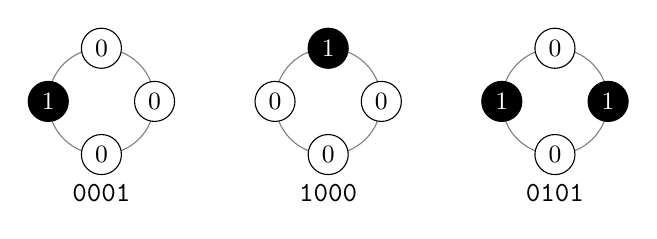
\begin{tikzpicture}[scale=.9]
 \foreach \offset/\bits/\labeltext in {0/{0,0,0,1}/{0001},3.2/{1,0,0,0}/{1000},6.4/{0,1,0,1}/{0101}} {
  \begin{scope}[xshift=\offset cm]
   \draw[gray] (0,0) circle (.75);
   \foreach \bit [count=\i from 0] in \bits {
    \ifnum\bit=1
     \node[circle,draw,fill=black,text=white,inner sep=2.5pt,font=\small] at ({90-90*\i}:.75) {1};
    \else
     \node[circle,draw,fill=white,inner sep=2.5pt,font=\small] at ({90-90*\i}:.75) {0};
    \fi
   }
   \node at (0,-1.3) {$\mathtt{\labeltext}$};
  \end{scope}
 }
\end{tikzpicture}
\caption{Reading clockwise from the top gives the displayed words. The
first two drawings represent the same necklace. The alternating necklace
on the right has only two distinct rotations.}
\label{fig:rings}
\end{figure}

Two words are \emph{rotation-equivalent} if one is a rotation of the
other. This is an equivalence relation: every word is equivalent to
itself, the relation is symmetric, and it is transitive. Its classes
partition all $2^n$ words. The set of necklaces is the \emph{orbit space}
$\mathcal N_n=\{0,1\}^n/C_n$.

\subsection{Least period and primitive necklaces}

The \emph{least spatial period} of $w$ is the smallest positive integer
$d$ such that $R^d w=w$. It divides $n$, and $w$ is a repetition of a
word of length $d$. This shortest block is a \emph{primitive root} of
the written word. Changing the starting position rotates that root, so
its necklace is well defined independently of the representative.

For example, $\word{001001001001}$ has least period $3$ and primitive
root $\word{001}$. Its necklace consists of three distinct words.
The word $\word{001001}$ is another repeated word; its length remains
$6$ even though its least period is $3$.

\begin{proposition}\label{prop:orbit-size}
A word of least spatial period $d$ has exactly $d$ distinct rotations.
\end{proposition}
\begin{proof}
The words $w,Rw,\ldots,R^{d-1}w$ are distinct by minimality of $d$,
and further rotations repeat them. Equivalently, the stabilizer of $w$
in $C_n$ has $n/d$ elements, so the orbit--stabilizer theorem gives
$|[w]|=n/(n/d)=d$.
\end{proof}

A necklace of length $n$ is \emph{primitive}, or \emph{aperiodic}, if
its least spatial period is $n$. Here ``aperiodic'' means that no smaller
rotational period exists. It says nothing about the temporal evolution
introduced below.

\section{Counting the necklaces}\label{sec:counting}

At length $4$ the six rotation classes are represented by
\[
 \word{0000},\ \word{0001},\ \word{0011},\
 \word{0101},\ \word{0111},\ \word{1111}.
\]
Their respective sizes are $1,4,4,2,4,1$, which sum to $16$.
Simply dividing $2^4$ by $4$ would be incorrect because some orbits
are shorter than others.

\subsection{Averaging fixed points}

Burnside's lemma counts orbits by averaging the numbers of objects fixed
by the group elements. A rotation through $k$ positions splits the $n$
positions into $\gcd(n,k)$ cycles. A word fixed by that rotation must
be constant on each such cycle, giving $2^{\gcd(n,k)}$ choices.
Therefore the number of binary necklaces of length $n$ is
\begin{equation}\label{eq:burnside}
 N(n)=\frac1n\sum_{k=0}^{n-1}2^{\gcd(n,k)}
 =\frac1n\sum_{d\mid n}\varphi(d)2^{n/d},
\end{equation}
where $\gcd(n,0)=n$ and $\varphi(d)$ is Euler's totient function, the
number of integers from $1$ to $d$ relatively prime to $d$.

The averaging can be justified directly. Count pairs $(w,R^k)$ for
which $R^kw=w$. An orbit of size $d$ contains $d$ words, each fixed
by $n/d$ rotations, so every orbit contributes exactly $n$ pairs.
The first sum in \eqref{eq:burnside} counts the same pairs by rotation.
The second groups rotations by their orders. At $n=4$ this gives
\[
 N(4)=\frac{16+2+4+2}{4}=6.
\]

\subsection{A consequence for primes}

If $p$ is prime, a length-$p$ word has least period $1$ or $p$.
The only period-one words are $\zero$ and $\one$, the constant-zero
and constant-one words. The other $2^p-2$ words occur in rotation
classes of size $p$. Hence
\[
 p\mid 2^p-2.
\]
This is the base-two case of Fermat's little theorem. The proof is a
partition argument: divisibility follows because a set has been divided
into equal-sized classes.

\section{Adjacent XOR and the binary Ducci map}\label{sec:ducci}

Addition modulo two has the table
\[
 \begin{array}{c|cc}
 +&0&1\\\hline
 0&0&1\\
 1&1&0
 \end{array}
\]
and is also called \emph{exclusive OR}, or XOR. Applying it coordinate
by coordinate turns binary words into the vector space $V_n=\F^n$,
where $\F$ is the field with two elements. In subset language, this
addition is symmetric difference:
$A_{u+v}=A_u\mathbin{\triangle}A_v$.

Define the \emph{adjacent-XOR map}
\begin{equation}\label{eq:ducci}
 D(w)=w+Rw,\qquad (Dw)_i=w_i+w_{i-1},
\end{equation}
with indices modulo $n$. Thus each new bit records whether a pair of
neighboring bits differs. For example,
\[
 \begin{array}{r@{\quad}l}
 w&\word{0001}\\
 Rw&\word{1000}\\\hline
 Dw&\word{1001}
 \end{array}
 \qquad\text{and hence}\qquad
 \overline D\neck{0001}=\neck{0011}.
\]
The notation $\overline D$ denotes the induced operation on necklaces.

This map is the \emph{binary Ducci map}. The usual Ducci operation
takes absolute differences of cyclically adjacent entries; on bits,
$|a-b|=a+b\pmod2$. Choosing the other neighbor reverses the spatial
convention. It gives $I+R^{-1}=R^{-1}(I+R)$, which induces exactly the
same map on rotation classes. Thus the necklace operation is independent
of this choice of direction. ``Adjacent XOR'' describes the rule;
``binary Ducci map'' places it in its established mathematical context.

\subsection{Why the operation is well defined}

A definition using a representative must give the same necklace no
matter which rotation is chosen. This follows from
\begin{equation}\label{eq:equivariance}
 D(R^j w)=R^jD(w).
\end{equation}
Indeed, $D=I+R$ commutes with every power of $R$. Consequently
$\overline D([w])=[Dw]$ is well defined. This is an example of an
\emph{equivariant} map descending to an orbit space.

Only \emph{adjacent} rotations define this particular rule. Replacing
$R$ by $R^k$ would in general give a different map. Also, the orbit
space of necklaces is not itself a vector space under an arbitrary
choice of representatives. At length $3$, for example, both
$\word{001}$ and $\word{010}$ represent the same necklace, but
\[
 \word{001}+\word{001}=\word{000},\qquad
 \word{010}+\word{001}=\word{011}.
\]
The output necklaces differ. The linear algebra takes place on words;
equivariance is what permits this particular map on necklaces.

\subsection{Repetition respects the dynamics}

If $d\mid n$, repeat a length-$d$ word $n/d$ times to obtain a
length-$n$ word. Every adjacent pair in the repeated word is the
corresponding pair in the shorter circular word, including at the
joins. Repetition therefore commutes with $R$ and $D$. A shorter
necklace and its repetitions have compatible trajectories, although
they belong to different spaces $\mathcal N_d$ and $\mathcal N_n$.

More generally, the least spatial period cannot increase under $D$:
if $R^dw=w$, then $R^dDw=Dw$. The output's least period divides $d$.
It may decrease, as in $\word{0101}\mapsto\word{1111}$.

\section{Predecessors, parity, and complementation}\label{sec:preimages}

The \emph{Hamming weight} $\wt(w)$ is the number of ones in a word.
Its parity is $\sum_iw_i$ in $\F$. Every adjacent-XOR output has
even weight, because each input bit contributes to two output positions:
\begin{equation}\label{eq:parity}
 \sum_i(Dw)_i=\sum_i(w_i+w_{i-1})=0.
\end{equation}
There is also a geometric interpretation. Ones in $Dw$ mark changes
between neighboring bits. Traveling once around a circle, the number
of changes from zero to one must equal the number from one to zero.

\begin{proposition}[The preimage criterion]\label{prop:preimages}
A word $y$ has a preimage under $D$ if and only if $\wt(y)$ is even.
When preimages exist, there are exactly two, and they are complements.
\end{proposition}
\begin{proof}
Necessity follows from \eqref{eq:parity}. Conversely, choose $w_0$
arbitrarily and use $w_i=y_i+w_{i-1}$ for $1\le i<n$. The remaining
equation $w_0+w_{n-1}=y_0$ holds precisely when $\sum_i y_i=0$.
Thus either choice of $w_0$ gives a solution. Changing that choice
changes every bit, so the two solutions are complements.
\end{proof}

Write $\overline w=w+\one$ for the \emph{complement}. Since
$D\one=\zero$, one has $D\overline w=Dw$. Complement is different
from additive inverse: in $\F^n$, every word is its own additive
inverse. The kernel of $D$ is $\{\zero,\one\}$, and its image is
the $(n-1)$-dimensional subspace of even-weight words.

On necklaces, an even-weight output has one or two distinct predecessor
vertices. To see why there are no more, rotate any predecessor so that
its image is a chosen representative $y$, and apply
Proposition~\ref{prop:preimages}. The two word solutions may lie in
the same necklace. For example,
\[
 D(\word{0101})=D(\word{1010})=\word{1111},
 \qquad\neck{0101}=\neck{1010}.
\]
Thus $\neck{1111}$ has just one predecessor necklace.
By contrast, the two predecessors of $\neck{0011}$ are
$\neck{0001}$ and $\neck{0111}$. An odd-weight necklace has none.
The term \emph{preimage} describes a relation, not a single inverse
function defined everywhere.

\subsection{Self-complementary necklaces}

A necklace is \emph{self-complementary} if $[\overline w]=[w]$:
some rotation exchanges all zeros with ones. For a word of least
spatial period $d$, this is equivalent to
\begin{equation}\label{eq:self-complement}
 d\text{ even},\qquad R^{d/2}w=\overline w.
\end{equation}
Indeed, if $R^sw=\overline w$, then $R^{2s}w=w$ but $R^sw\ne w$.
In the cyclic group of shifts modulo $d$, the only element of order
two is the half-turn $d/2$. Conversely, that half-turn establishes
self-complementarity.

The primitive block therefore has complementary halves. The full
length-$n$ word need not: $\word{0101}$ is self-complementary, but
its two length-two halves are both $\word{01}$. Its primitive block
$\word{01}$ has the complementary halves $\word{0}$ and $\word{1}$.

\section{From trajectories to functional graphs}\label{sec:graphs}

Draw one vertex for each necklace of length $n$, and one directed edge
$[w]\to[Dw]$. The result is a \emph{functional digraph}, denoted
$\mathcal Q_n$. Every vertex has exactly one outgoing edge, although
it may have zero, one, or two incoming edges. Self-loops are retained.
The edges record adjacent XOR on subsets after rotations have been
identified; they do not describe subset inclusion.

Starting at a vertex and following its outgoing edges gives its
\emph{forward trajectory}. Because the graph is finite, some vertex
eventually repeats, after which the trajectory follows a directed cycle.
The earlier vertices form the transient part of that trajectory.

A \emph{weakly connected component} is a maximal set of vertices
connected when edge directions are ignored. Each such component has
exactly one directed cycle: an edge joins two vertices with the same
eventual cycle, so two different eventual cycles cannot lie in one
component. The remaining vertices form rooted trees directed toward
the cycle. Such a component is also the \emph{basin of attraction} of
its cycle. It usually branches and is not merely a path.

The \emph{cycle length} is the number of necklaces on the cycle. The
\emph{depth} of a transient vertex is the number of steps needed to
reach the cycle; cycle vertices have depth zero. A vertex with no
predecessors is a leaf of an incoming tree. At the cycle root, the
incoming cycle edge is distinct from any incoming tree edges.

\subsection{Two components with the same shape}

At $n=3$, all four necklaces and their images are as follows.
\begin{table}[htbp]
\centering
\renewcommand{\arraystretch}{1.2}
\begin{tabular}{@{}cccc@{}}
\toprule
Necklace & Number of represented words & Image & Component\\
\midrule
$\neck{000}$ & $1$ & $\neck{000}$ & A\\
$\neck{111}$ & $1$ & $\neck{000}$ & A\\
$\neck{011}$ & $3$ & $\neck{011}$ & B\\
$\neck{001}$ & $3$ & $\neck{011}$ & B\\
\bottomrule
\end{tabular}
\caption{The complete necklace dynamics at length $3$.}
\label{tab:three}
\end{table}
Both components consist of one looped root with one leaf pointing to it.
They are \emph{isomorphic}: a bijection between their vertices preserves
the directed edges. There are therefore two components but only one
\emph{graph type}.

Nevertheless, component A represents two words, while component B
represents six. To retain this information, give a necklace vertex the
weight $|[w]|$, its number of represented words, and define the
\emph{mass} of a component $C$ by
\begin{equation}\label{eq:mass}
 \lVert C\rVert=\sum_{[w]\in V(C)}|[w]|.
\end{equation}
Unweighted graph isomorphism need not preserve mass.

\subsection{A complete branching example}

At $n=4$, all six necklaces lie in the component shown in
Figure~\ref{fig:four}. The zero necklace is its only cycle vertex.
Its two depth-four leaves are distinct, even though their subsequent
trajectories agree.

\begin{figure}[htbp]
\centering
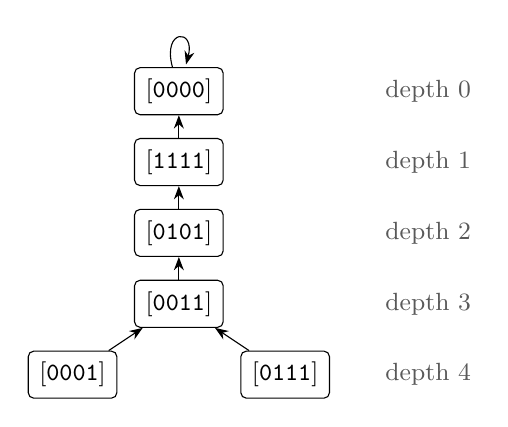
\begin{tikzpicture}[>=Stealth,
 v/.style={draw,rounded corners=2pt,inner sep=4pt,font=\small},
 every edge/.style={draw,->}]
 \node[v] (a) at (0,0) {$\neck{0000}$};
 \node[v] (b) at (0,-.9) {$\neck{1111}$};
 \node[v] (c) at (0,-1.8) {$\neck{0101}$};
 \node[v] (d) at (0,-2.7) {$\neck{0011}$};
 \node[v] (e) at (-1.35,-3.6) {$\neck{0001}$};
 \node[v] (f) at (1.35,-3.6) {$\neck{0111}$};
 \path (a) edge[loop above] (a) (b) edge (a) (c) edge (b)
 (d) edge (c) (e) edge (d) (f) edge (d);
 \foreach \y/\depth in {0/0,-.9/1,-1.8/2,-2.7/3,-3.6/4}
  \node[anchor=west,font=\small,text=black!65] at (2.5,\y) {depth $\depth$};
\end{tikzpicture}
\caption{The entire graph $\mathcal Q_4$. The vertex weights are
$1,1,2,4,4,4$, from the root downward, summing to $16$.}
\label{fig:four}
\end{figure}

Reading total indegrees by depth gives the branching sequence
\[
 2,1,1,2,0.
\]
The first $2$ counts the root's loop and its incoming tree edge.
The last $0$ records the leaves. For a tree whose branching is uniform
at each depth, these numbers describe its shape. Such uniformity is
additional structure; it does not hold for every functional graph.
One can encode the example as $G_1\text{-}21120$, where the subscript
is the cycle length and the symbols form a word over $\{0,1,2\}$.

\subsection{Accounting for the power set}

Every word belongs to one rotation class, and every necklace belongs
to one graph component. Taking the union of the rotation classes in
each component therefore partitions $\mathcal P(X_n)$. In particular,
\begin{equation}\label{eq:accounting}
 \sum_{C\text{ component of }\mathcal Q_n}\lVert C\rVert=2^n.
\end{equation}
Grouping isomorphic components is a further classification, not an
identification of their subsets. A complete description should retain
the graph types, their component multiplicities, and the represented
word counts. These are three different pieces of information.

\section{Why odd lengths and powers of two behave differently}\label{sec:lengths}

The simplest structural results already distinguish two large families
of lengths. They follow from the same linear map $D=I+R$.

\subsection{Odd lengths: cycles with one leaf at each vertex}

\begin{proposition}\label{prop:odd}
If $n$ is odd, every even-weight word is periodic under $D$, and every
odd-weight word enters the periodic set after one step. Every component
of $\mathcal Q_n$ is a directed cycle with one leaf attached to each
cycle vertex.
\end{proposition}
\begin{proof}
Let $E$ be the subspace of even-weight words. It is preserved by $D$.
The kernel of $D$ consists of $\zero$ and $\one$, but $\one$ has odd
weight. Thus the restriction $D:E\to E$ is injective, and hence
bijective because $E$ is finite. Every element of $E$ is consequently
periodic.

An even-weight word has two complementary preimages, exactly one even
and one odd. The even predecessor lies on its periodic orbit. The odd
predecessor has no predecessors itself. This remains true after taking
rotation classes: parity is preserved by rotation, and an equivariant
bijection on $E$ gives a bijection on its necklaces.
\end{proof}

For example, at $n=5$ the nonzero periodic necklaces form the cycle
\begin{equation}\label{eq:five-cycle}
 \neck{00011}\longrightarrow\neck{00101}
 \longrightarrow\neck{01111}\longrightarrow\neck{00011}.
\end{equation}
Their attached leaves are, respectively, $\neck{00001}$,
$\neck{00111}$, and $\neck{01011}$. The other component consists of
$\neck{11111}\to\neck{00000}$ with a loop at $\neck{00000}$.
The two graph types are $G_1\text{-}20$ and $G_3\text{-}20$.
The component masses are $2$ and $6\cdot5=30$, accounting for all
$32$ words.

\subsection{Powers of two: eventual extinction}

Over $\F$, the middle term in a square vanishes:
\[
 (I+R)^2=I+2R+R^2=I+R^2.
\]
Repeated squaring gives $(I+R)^{2^a}=I+R^{2^a}$ for every nonnegative
integer $a$. Consequently:

\begin{proposition}\label{prop:power-two}
If $n=2^a$, every word reaches zero after at most $n$ steps. The
graph $\mathcal Q_n$ has one component, whose maximum transient
depth is exactly $n$.
\end{proposition}
\begin{proof}
Since $R^n=I$,
\[
 D^n=(I+R)^n=I+R^n=0.
\]
All necklaces therefore reach $[\zero]$, proving connectedness.
To see that depth $n$ is attained, let $e_0$ be the word with a single
one at position zero. Binary expansion of the exponent gives
\[
 (I+R)^{n-1}=\prod_{j=0}^{a-1}(I+R^{2^j})
 =I+R+\cdots+R^{n-1}.
\]
Thus $D^{n-1}e_0=\one\ne\zero$, and the next step is zero.
This also covers $n=1$, using the empty product $I$.
\end{proof}

In particular, the tree at length $2^a$ has $2^a+1$ levels when the
root is included. Figure~\ref{fig:four} illustrates the case $a=2$.

\begin{corollary}\label{cor:connected}
The graph $\mathcal Q_n$ is connected if and only if $n$ is a power
of two, including $n=1$.
\end{corollary}
\begin{proof}
Only the converse remains. If $n$ has an odd divisor $m>1$, choose
a nonzero even-weight word of length $m$. It is periodic by
Proposition~\ref{prop:odd}. Repeating it to length $n$ preserves its
periodicity and gives a nonzero periodic word. Its necklace lies on
a cycle distinct from $[\zero]$, so there is more than one component.
\end{proof}

\section{Reflection is a separate symmetry}\label{sec:reflection}

Let $J$ reverse a written word. Reversing the order around the circle
is different from exchanging zeros and ones. For example, complement
changes the weight from $k$ to $n-k$, whereas reflection preserves it.

A necklace is \emph{achiral} if its reflection belongs to the same
rotation class, $[Jw]=[w]$. Otherwise it is \emph{chiral} and has a
distinct mirror-image necklace. If reflections as well as rotations
are identified, the resulting objects are \emph{binary bracelets},
the orbits of a dihedral-group action. Here the vertices remain
necklaces, so distinct mirror images remain distinct vertices.

A \emph{palindrome} is a written word equal to its reversal. A
palindromic representative guarantees achirality, but the converse
fails at even lengths. The necklace $\neck{0101}$ is achiral because
its reversal is $\word{1010}$, a rotation. Neither of its two written
representatives is a palindrome. Geometrically, an axis of reflection
may pass through beads as well as through gaps.

Reflection induces an automorphism of the necklace graph. On words,
\[
 JR=R^{-1}J,\qquad JD=R^{-1}DJ.
\]
The extra rotation disappears on necklaces, so
$\overline J\,\overline D=\overline D\,\overline J$. Thus reflection
maps a component either to itself or to a distinct isomorphic component.

An invariant component need not have every vertex individually fixed
by reflection. At length $6$, the two distinct chiral necklaces
\[
 \neck{001011}\quad\text{and}\quad\neck{001101}
\]
both map to the achiral necklace $\neck{010111}$. Their reflections
are paired within a single component containing both chiral and
achiral vertices. The commutation relation implies that an achiral
necklace always has an achiral image; it does not imply that all its
preimages are achiral.

\section{Space--time patterns and cycles with drift}\label{sec:patterns}

A trajectory can be displayed as an array: write the initial word in
row zero, its image in row one, and continue downward. Repeat every
row horizontally to display its circular boundary condition. If
$a(i,t)$ is the bit at position $i$ and time $t$, then
\begin{equation}\label{eq:spacetime}
 a(i,t+1)=a(i,t)+a(i-1,t)\pmod2,
 \qquad a(i+n,t)=a(i,t).
\end{equation}
This is a \emph{space--time diagram} of a one-dimensional additive
cellular automaton. Replacing zeros and ones by white and black squares
gives a coloring of the square grid obeying the same local rule.

\subsection{Pascal's triangle modulo two}

Since $I$ and $R$ commute, the binomial theorem gives
\begin{equation}\label{eq:pascal}
 D^t=(I+R)^t=\sum_{j=0}^{t}\binom tj R^j,
\end{equation}
with coefficients reduced modulo two. Starting from a single one,
the nonzero coefficients form Pascal's triangle modulo two, as in
Figure~\ref{fig:spacetime}. On a circle, contributions whose positions
agree modulo $n$ add modulo two and may cancel. The familiar growing
triangle describes the initial rows before this circular overlap.

\begin{figure}[htbp]
\centering
\newcommand{\pixelrow}[2]{%
 \foreach \bit [count=\col from 0] in {#2}{%
  \ifnum\bit=1\fill (\col,-#1) rectangle ++(1,-1);\fi}}
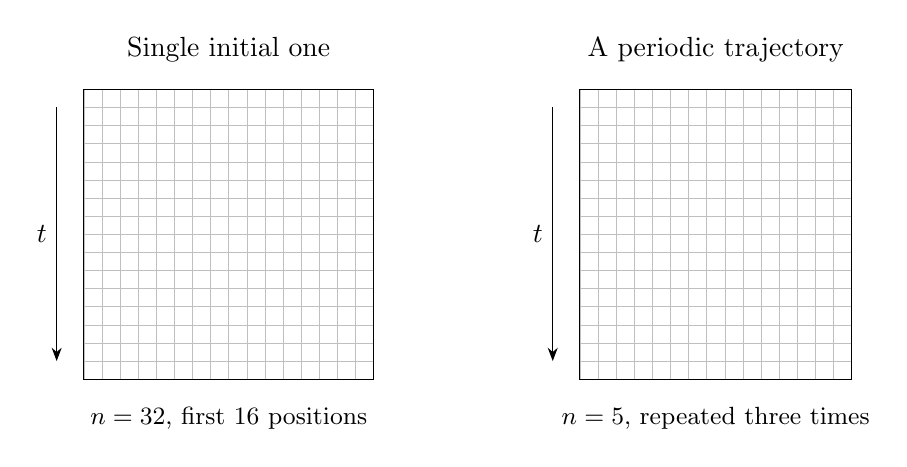
\begin{tikzpicture}[x=.23cm,y=.23cm,>=Stealth]
 \begin{scope}
  \pixelrow{0}{1,0,0,0,0,0,0,0,0,0,0,0,0,0,0,0}
\pixelrow{1}{1,1,0,0,0,0,0,0,0,0,0,0,0,0,0,0}
\pixelrow{2}{1,0,1,0,0,0,0,0,0,0,0,0,0,0,0,0}
\pixelrow{3}{1,1,1,1,0,0,0,0,0,0,0,0,0,0,0,0}
\pixelrow{4}{1,0,0,0,1,0,0,0,0,0,0,0,0,0,0,0}
\pixelrow{5}{1,1,0,0,1,1,0,0,0,0,0,0,0,0,0,0}
\pixelrow{6}{1,0,1,0,1,0,1,0,0,0,0,0,0,0,0,0}
\pixelrow{7}{1,1,1,1,1,1,1,1,0,0,0,0,0,0,0,0}
\pixelrow{8}{1,0,0,0,0,0,0,0,1,0,0,0,0,0,0,0}
\pixelrow{9}{1,1,0,0,0,0,0,0,1,1,0,0,0,0,0,0}
\pixelrow{10}{1,0,1,0,0,0,0,0,1,0,1,0,0,0,0,0}
\pixelrow{11}{1,1,1,1,0,0,0,0,1,1,1,1,0,0,0,0}
\pixelrow{12}{1,0,0,0,1,0,0,0,1,0,0,0,1,0,0,0}
\pixelrow{13}{1,1,0,0,1,1,0,0,1,1,0,0,1,1,0,0}
\pixelrow{14}{1,0,1,0,1,0,1,0,1,0,1,0,1,0,1,0}
\pixelrow{15}{1,1,1,1,1,1,1,1,1,1,1,1,1,1,1,1}
  \draw[step=1,black!25,very thin] (0,0) grid (16,-16);
  \draw (0,0) rectangle (16,-16);
  \node[anchor=south] at (8,1) {Single initial one};
  \node[anchor=north,font=\small] at (8,-17) {$n=32$, first $16$ positions};
  \draw[->] (-1.5,-1) -- (-1.5,-15) node[midway,left] {$t$};
 \end{scope}
 \begin{scope}[xshift=6.3cm]
  \pixelrow{0}{0,0,0,1,1,0,0,0,1,1,0,0,0,1,1}
\pixelrow{1}{1,0,0,1,0,1,0,0,1,0,1,0,0,1,0}
\pixelrow{2}{1,1,0,1,1,1,1,0,1,1,1,1,0,1,1}
\pixelrow{3}{0,0,1,1,0,0,0,1,1,0,0,0,1,1,0}
\pixelrow{4}{0,0,1,0,1,0,0,1,0,1,0,0,1,0,1}
\pixelrow{5}{1,0,1,1,1,1,0,1,1,1,1,0,1,1,1}
\pixelrow{6}{0,1,1,0,0,0,1,1,0,0,0,1,1,0,0}
\pixelrow{7}{0,1,0,1,0,0,1,0,1,0,0,1,0,1,0}
\pixelrow{8}{0,1,1,1,1,0,1,1,1,1,0,1,1,1,1}
\pixelrow{9}{1,1,0,0,0,1,1,0,0,0,1,1,0,0,0}
\pixelrow{10}{1,0,1,0,0,1,0,1,0,0,1,0,1,0,0}
\pixelrow{11}{1,1,1,1,0,1,1,1,1,0,1,1,1,1,0}
\pixelrow{12}{1,0,0,0,1,1,0,0,0,1,1,0,0,0,1}
\pixelrow{13}{0,1,0,0,1,0,1,0,0,1,0,1,0,0,1}
\pixelrow{14}{1,1,1,0,1,1,1,1,0,1,1,1,1,0,1}
\pixelrow{15}{0,0,0,1,1,0,0,0,1,1,0,0,0,1,1}
  \draw[step=1,black!25,very thin] (0,0) grid (15,-16);
  \draw (0,0) rectangle (15,-16);
  \node[anchor=south] at (7.5,1) {A periodic trajectory};
  \node[anchor=north,font=\small] at (7.5,-17) {$n=5$, repeated three times};
  \draw[->] (-1.5,-1) -- (-1.5,-15) node[midway,left] {$t$};
 \end{scope}
\end{tikzpicture}
\caption{Rows $t=0,\ldots,15$, with black for $1$ and white for $0$.
Left: the first sixteen rows of Pascal's triangle modulo two; the omitted
sixteen spatial positions are zero in all these rows. Right: evolution
from $\word{00011}$, repeated horizontally. Its necklace has period $3$,
but the written row first returns at time $15$.}
\label{fig:spacetime}
\end{figure}

\subsection{A necklace can return before its written word}

Spatial repetition and temporal repetition are different. A necklace
on a cycle returns after some least number $T$ of steps, but a chosen
word may return rotated:
\begin{equation}\label{eq:drift}
 D^T w=R^s w.
\end{equation}
If $d$ is the word's least spatial period, the \emph{drift} $s$ is
well defined modulo $d$. For example,
\[
 \word{011}\xrightarrow{D}\word{110}
 \xrightarrow{D}\word{101}\xrightarrow{D}\word{011}.
\]
These are three different words representing the same necklace.
The necklace is a fixed point, with $T=1$, even though the word has
temporal period $3$. Here $d=3$ and $s=2$ for our right-rotation
convention.

More generally, the least temporal period of the word itself is
\begin{equation}\label{eq:word-period}
 \tau=T\frac d{\gcd(d,s)}.
\end{equation}
To prove this, any return of the word must first be a return of its
necklace, so its time is a multiple of $T$. After $kT$ steps,
commutation gives $D^{kT}w=R^{ks}w$. The least positive $k$ with
$d\mid ks$ is $d/\gcd(d,s)$. When $s=0$, the convention
$\gcd(d,0)=d$ gives $\tau=T$.

At $n=5$, take $w=\word{00011}$. The necklace cycle in
\eqref{eq:five-cycle} has length $T=3$, while
\[
 D^3(\word{00011})=\word{00110}=R^4(\word{00011}).
\]
Thus $d=5$, $s=4$, and $\tau=15$. The right panel of
Figure~\ref{fig:spacetime} displays these fifteen steps and the
returning row.

If the starting word is periodic, extend the array periodically in
time as well as space. Equation~\eqref{eq:drift} says
\[
 a(i,t+T)=a(i-s,t),
 \qquad a(i+s,t+T)=a(i,t).
\]
The array is invariant under the two translations $(d,0)$ and
$(s,T)$ in the space--time plane. These generate a \emph{period
lattice}. A fundamental repeating region can consequently be skew:
the necklace cycle need not give a rectangular tile of height $T$.
A rectangular repeat has height $\tau$. This distinction explains
how a short cycle of circular patterns can generate a much taller
pattern in fixed coordinates.

\section{Toward an algebraic classification}\label{sec:algebra}

The examples suggest three questions for each length $n$:
which graph types occur, how many components have each type, and how
many subsets each component represents? Choosing representatives is
one way to display the answer, but it is not part of the definition
of a partition or a requirement for proving completeness.

The first algebraic step is to encode a word as a polynomial,
\[
 w_0w_1\cdots w_{n-1}
 \longleftrightarrow w_0+w_1x+\cdots+w_{n-1}x^{n-1}.
\]
Coefficients lie in $\F$, and exponents are taken cyclically, using
$x^n=1$. Thus the word space can be written as
\begin{equation}\label{eq:polynomial-space}
 V_n=\F[x]/(x^n+1),\qquad Rw=xw,\qquad Dw=(1+x)w.
\end{equation}
The plus sign in $x^n+1$ is also a minus sign in characteristic two.
Rotation and evolution have become multiplication by two fixed
polynomials. This representation is part of the established algebraic
theory of additive cellular automata and Ducci sequences
\cite{MartinOdlyzkoWolfram,MisiurewiczStevensThomas}.

Write uniquely
\begin{equation}\label{eq:odd-part}
 n=2^a m=qm,\qquad a\ge0,\qquad m\text{ odd}.
\end{equation}
Here $a$ is the number of factors of two in $n$, and $m$ is its odd
part. For example, $40=2^3\cdot5$. Repeated squaring gives
\begin{equation}\label{eq:factorization}
 x^n+1=(x^m+1)^q=(x+1)^q Q_m(x)^q,
 \qquad Q_m(x)=\frac{x^m+1}{x+1}.
\end{equation}
Since $m$ is odd, the factors $x+1$ and $Q_m$ are relatively prime.
The Chinese remainder theorem separates two coordinates:
\[
 V_n\simeq
 \underbrace{\F[y]/(y^q)}_{\text{transient coordinate}}
 \ \oplus\
 \underbrace{\F[x]/Q_m(x)^q}_{\text{periodic coordinate}},
 \qquad y=x+1.
\]
In the first coordinate, $D$ multiplies by $y$, and $y^q=0$, so every
value eventually vanishes. In the second, $1+x$ is invertible, so
evolution permutes a finite set of values. This is an algebraic
explanation of the trees and cycles in the graph.

For a power of two, $m=1$ and $Q_m=1$, so the periodic coordinate
contains only zero. For odd $n$, $q=1$, so the transient coordinate
disappears after one step. These are exactly the two situations
proved elementarily in Section~\ref{sec:lengths}.

The companion paper \emph{The Partitioning of Power Sets Into Graphs}
develops this decomposition into a classification of the necklace
components. Among its consequences are a common tree depth $q$,
identical level-regular trees at the cycle vertices of a component,
and formulas that describe every length $m2^a$ from finite algebraic
data associated with the odd part $m$. Its counting formulas accompany
a proof of disjointness and exhaustiveness, accounting for all $2^n$
subsets.

Necklaces, dynamical components, and graph types organize different
levels of structure. A necklace forgets a starting position. A
component collects every necklace attracted to one cycle. A graph
type retains the arrangement of edges while discarding vertex labels.
Keeping these levels distinct allows both the geometry of the
dynamics and the exact partition of the power set to be described.

\section*{Further reading}

Binary necklaces are standard objects in combinatorics on words;
\cite{DegniDrisko} provides one entry into their literature. The
binary Ducci map and its finite-field formulation are treated in
\cite{MisiurewiczStevensThomas}, and polynomial methods for additive
cellular automata in \cite{MartinOdlyzkoWolfram}. Rotation quotients
of cellular-automaton graphs, for a broader range of local rules,
are considered in \cite{FratiPetakCheney}. These perspectives place
the elementary constructions above within established mathematical
frameworks.

\begin{thebibliography}{9}

\bibitem{DegniDrisko}
C.~Degni and A.~A.~Drisko,
\emph{Gray-ordered binary necklaces},
The Electronic Journal of Combinatorics \textbf{14} (2007), no.~1,
Research Paper~7.
\href{https://doi.org/10.37236/926}{doi:10.37236/926}.

\bibitem{MisiurewiczStevensThomas}
M.~Misiurewicz, J.~G.~Stevens, and D.~M.~Thomas,
\emph{Iterations of linear maps over finite fields},
Linear Algebra and its Applications \textbf{413} (2006), no.~1,
218--234.
\href{https://doi.org/10.1016/j.laa.2005.09.002}{doi:10.1016/j.laa.2005.09.002}.

\bibitem{MartinOdlyzkoWolfram}
O.~Martin, A.~M.~Odlyzko, and S.~Wolfram,
\emph{Algebraic properties of cellular automata},
Communications in Mathematical Physics \textbf{93} (1984), no.~2,
219--258.
\href{https://doi.org/10.1007/BF01223745}{doi:10.1007/BF01223745}.

\bibitem{FratiPetakCheney}
L.~Frati, C.~Petak, and N.~Cheney,
\emph{Networks of binary necklaces induced by elementary cellular
automata rules}, 2024.
\href{https://arxiv.org/abs/2409.04780}{arXiv:2409.04780}.

\end{thebibliography}
\end{document}
